\section{Stoffklassen}

\small{\begin{tabularx}{\columnwidth}{|l|l|l|X|}
		\hline
		\textbf{Stoffklasse} & \textbf{Bindungstyp} & \textbf{Beispiel} & \textbf{Eigenschaften} \\
		\hline
		Salze & \makecell[l]{\textbf{Ionenbindung} \\ Metall - Nichtmetall} & NaCl, CaCl\textsubscript{2} & Spröde, \newline hohe Schmelzpunkte, lösen sich oft gut in Wasser \\
		\hline
		Metalle & \makecell[l]{\textbf{Metallbindung} \\ Metall - Metall} & Cu, Fe, Al & Leitfähig, glänzend \\
		\hline
		\makecell[l]{Molekulare \\ Stoffe}& \makecell[l]{\textbf{Kovalente Bindung} \\ Nichtmetall - Nichtmetall} & H\textsubscript{2}O, CO\textsubscript{2}, CH\textsubscript{4} & niedrige Schmelz- und Siedepunkte, oft gasförmig oder flüchtig \\
		\hline
\end{tabularx}}

\subsection{Moleküle}
Ein Molekül ist ein abgeschlossener Atomverbund aus reinen Nichtmetallen.
Die Polarität eines Moleküls ist abhängig von der Polarität der Bindungen und der asymmetrie der Geometrie. (hierbei ist Symmetrie wichtiger) 

$$ \boxed{\Delta EN = |EN(Atom 1) - EN(Atom 2)|}$$

$$\boxed{\Delta EN \le 0.4 \text{: unpolare Bindung}} \qquad \boxed{0.4 < \Delta EN \le 1.5 \text{: polare Bindung}} $$

\subsubsection{ZMK - Zwischenmolekularkräfte}

\small{\begin{tabularx}{\columnwidth}{|l|l|X|}
		\hline
		\textbf{Art} & \textbf{Eigenschaft} & \textbf{Grad} \\
		\hline
		Van der Waals & wirken zwischen allen Molekülen &  schwach\\
		\hline
		Dipol-Dipol & ein permanenter Dipol (Polar und Asymmterisch) & mittel \\
		\hline
		Wasserstoffbrücken & freies Elektron vom H-Atom an N, O, F Atom gebunden & stark \\ 
		\hline
\end{tabularx}}

\vspace{0.2cm}

Die Dipol-Dipol- und die Wasserstoffbrücken-Kraft wirken erst, wenn das Molekül polarisiert ist, sonst wirkt nur die Van der Waals Kraft.
Die Van der Waals Kraft wird mit höherer Anzahl Elektronen grösser.

Die ZMK ist unter anderem für die Side- und Schmelpunkte und Löslichkeit verantwortlich.

Ein molekularer Stoff ist löslich, wenn er dieselben ZMKs wie das Lösungsmittel aufweist.

\subsection{Bindungswinkel}
\begin{center}
	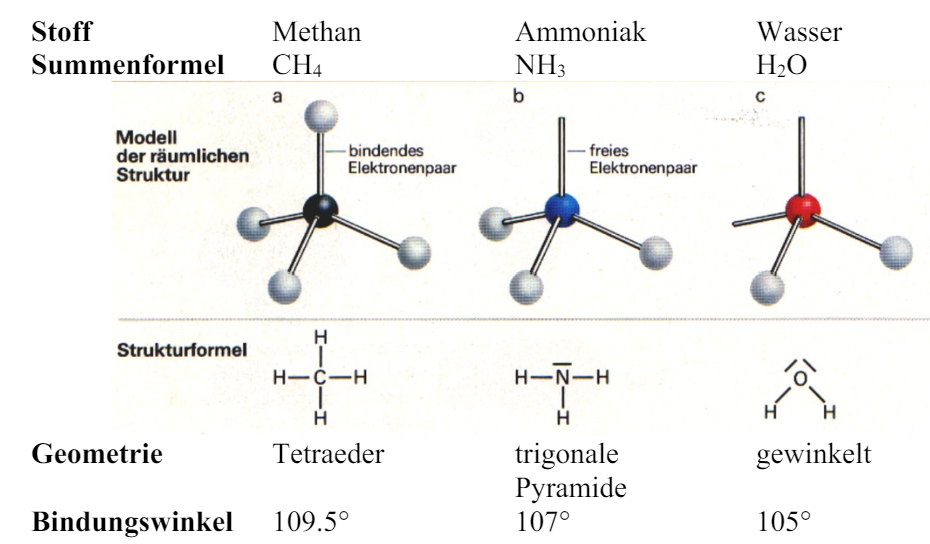
\includegraphics[height=4cm]{images/Winkel.png}
\end{center}


\subsection{Salze}
Bei der Reaktion bilden sich Ionen in einem Gitter aus "\text{unendlich}" vielen Ionen zusammen (= \textbf{Ionengitter}).
\begin{itemize}
	\item Kation: positiv (meist metallisch)
	\item Anion: negativ (immer nichtmetallisch, kann auch als ganzes Molekül vorkommen)
\end{itemize}

Die Salzformel beschreibt das Verhältnis zwischen Anion und Kation

\textbf{Bestimmung der Salzformel:}
\begin{enumerate}
	\item Ionen erfüllen Edelgasregel $\rightarrow$ Ionenladung (z.B. Na $\rightarrow$ Na\textsuperscript{+}, Al $\rightarrow$ Al\textsuperscript{3+}, Cl $\rightarrow$ Cl\textsuperscript{-}, O $\rightarrow$ O\textsuperscript{2-})
	\item Ladungsausgleich der Ionen $\rightarrow$ Zahlenverhältnis der Ionen (z.B. 2 $\cdot$ Al\textsuperscript{3+} + 3 $\cdot$ O\textsuperscript{2-} $\rightarrow$ Al\textsubscript{2}O\textsubscript{3})
\end{enumerate}
Die \textbf{Löslichkeit} eines Salzes ist abhängig von der Ionenladung:
(gut: Na\textsuperscript{+}Cl\textsuperscript{-}, schlecht: Ca\textsuperscript{2+}CO\textsubscript{3}\textsuperscript{2-})

\subsection{Metalle und Halbmetalle}
 \subsubsection{Metalle}
  Metalle besitzen durch delokalisierte Elektronenwolken (VE) dh. freie Ladungsträger, dies führt zu gute Wärme- und el. Leitfähigkeit, Verformbarkeit. Valenzband Vb nicht ganz gefüllt. \newline
  $\rightarrow$ Elektronen können sich im Band bewegen \newline
  \textbf{Leitfähigkeit:}
	\begin{itemize}
		\item nimmt mit steigender Temperatur ab
		\item die Bewegung der Atomrümpfe erhöht sich
		\item weniger Platz für die Elektronenbewegung
	\end{itemize}
	\smallskip

\subsubsection{Halbmetalle}
 Halbmetalle haben weder Elektronenwolken noch überlappende Energieniveaus, Nähe vom Valenz- und Leitungsband ermöglichen aber ein Überspringen \newline
\textbf{Leitfähigkeit:}
	\begin{itemize}
		\item nimmt mit steigender Temperatur stark zu
		\item die Elektronen springen viel zahlreicher auf das Leitungband über
		\item Platz für Elektronenbewegung im Leitungsband
	\end{itemize}
	
\subsection{Dotierung von Halbmetallen}
Dotierung $\rightarrow$ Einbringen von Fremdatomen ins Atomgitter eines Halbleiters
\begin{itemize}
	\item \textbf{n-Halbleiter}
	\item[] z.B. einzelne As-Atome im Si-Gitter(1:10'000'000)
	\item[] Ein \tikz[baseline=(text.base)]\node[fill=orange, fill opacity=0.3, text opacity=1, rounded corners, inner sep=2pt, minimum height=5pt] (text) {\textit{überschüssiges}}; 
	Elektron pro As-Atom $\Rightarrow$ Leitfähigkeit: Elektron von As-Atom kann ins Leitungsband von Si überspringen und sich frei bewegen
	\item \textbf{p-Halbleiter}
	\item[] z.B. einzelne B-Atome im Si-Gitter(1:1'000'000)
	\item[] Ein \tikz[baseline=(text.base)]\node[fill=orange, fill opacity=0.3, text opacity=1, rounded corners, inner sep=2pt, minimum height=5pt] (text) {\textit{fehlendes}}; Elektron pro B-Atom $\Rightarrow$ Leitfähigkeit: Elektronen aus dem vollen Valenzband von Si können in diese ``Lücke'' springen und sich frei bewegen
\end{itemize}
